\documentclass[a4paper,11pt]{jsarticle} 
\usepackage{url}
\usepackage{seiritz}
\pagestyle{fancy}
  \cfoot{\thepage}
  \renewcommand{\headrulewidth}{0pt}

\begin{document}
%本文
\begin{titlepage}
  \begin{center}
    \vspace*{\stretch{1}}
    {\Huge\gt テスト演習}\\ \vspace{\baselineskip}
    \textup{\large 実施日:2023年10月21日}\\ \vspace{\stretch{1}}
  \end{center}
  \vfill
  \hfill {最終更新日:\today}
\end{titlepage}

\qPart
%!TEX root = *.tex
%%%%%%%%%%%%%%%%%%
% カウンタのリセット
% 問題文
滑車と糸の質量は無視できるものとし,重力加速度を\g とする.

\begin{enumerate}[〔A〕]
  \setlength{\leftskip}{-1.5zw}
  \setlength{\itemindent}{1zw}\setlength{\labelsep}{0.5zw}
  \setlength{\labelwidth}{1zw}\setlength{\leftmargin}{1zw}
  \setlength{\itemsep}{0.5\baselineskip}
  \item 図1のように,なめらかに回る定滑車に伸縮しない糸をかけて,糸の一方に質量$m_1$のおもりA,他方に質量$m_2$のおもりBをつけて静かに放した.
  \begin{enumerate}[(1)]
    \setlength{\leftskip}{-2.5zw}
    \setlength{\itemindent}{1zw}\setlength{\labelsep}{1zw}
    \setlength{\labelwidth}{1zw}
    \item $m_1 > m_2$のとき,おもりAが下降する加速度の大きさを求めよ.
    \item 糸に働く張力の大きさを求めよ.
    \item $m_1 + m_2 = \text{一定}$として,糸の張力を最大にする$m_1$と$m_2$の関係を求めよ.
  \end{enumerate}
  \item 次に,図2のように定滑車の一方に質量$3M$のおもりCを,他方に動滑車をつり下げて,動滑車には質量$2M$のおもりDと質量$M$のおもりEをつり下げた.C,D,Eを同時に静かに放した.
  \begin{enumerate}[(1)]
    \setlength{\leftskip}{-2.5zw}
    \setlength{\itemindent}{1zw}\setlength{\labelsep}{1zw}
    \setlength{\labelwidth}{1zw}
    \item おもりC,D,Eの加速度の大きさを求めよ.
    \item おもりD,E間の糸に働く張力の大きさを求めよ.
    \item おもりD,EはそのままでおもりCを$\C^\prime$に換えると,$\C^\prime$,D,Eを同時に静かに放しても,おもりは静止したまま動かなかった.
    このときのおもり$\C^\prime$の質量を求めよ.
  \end{enumerate}
\end{enumerate}

\begin{figure}[htbp]
  \centering
  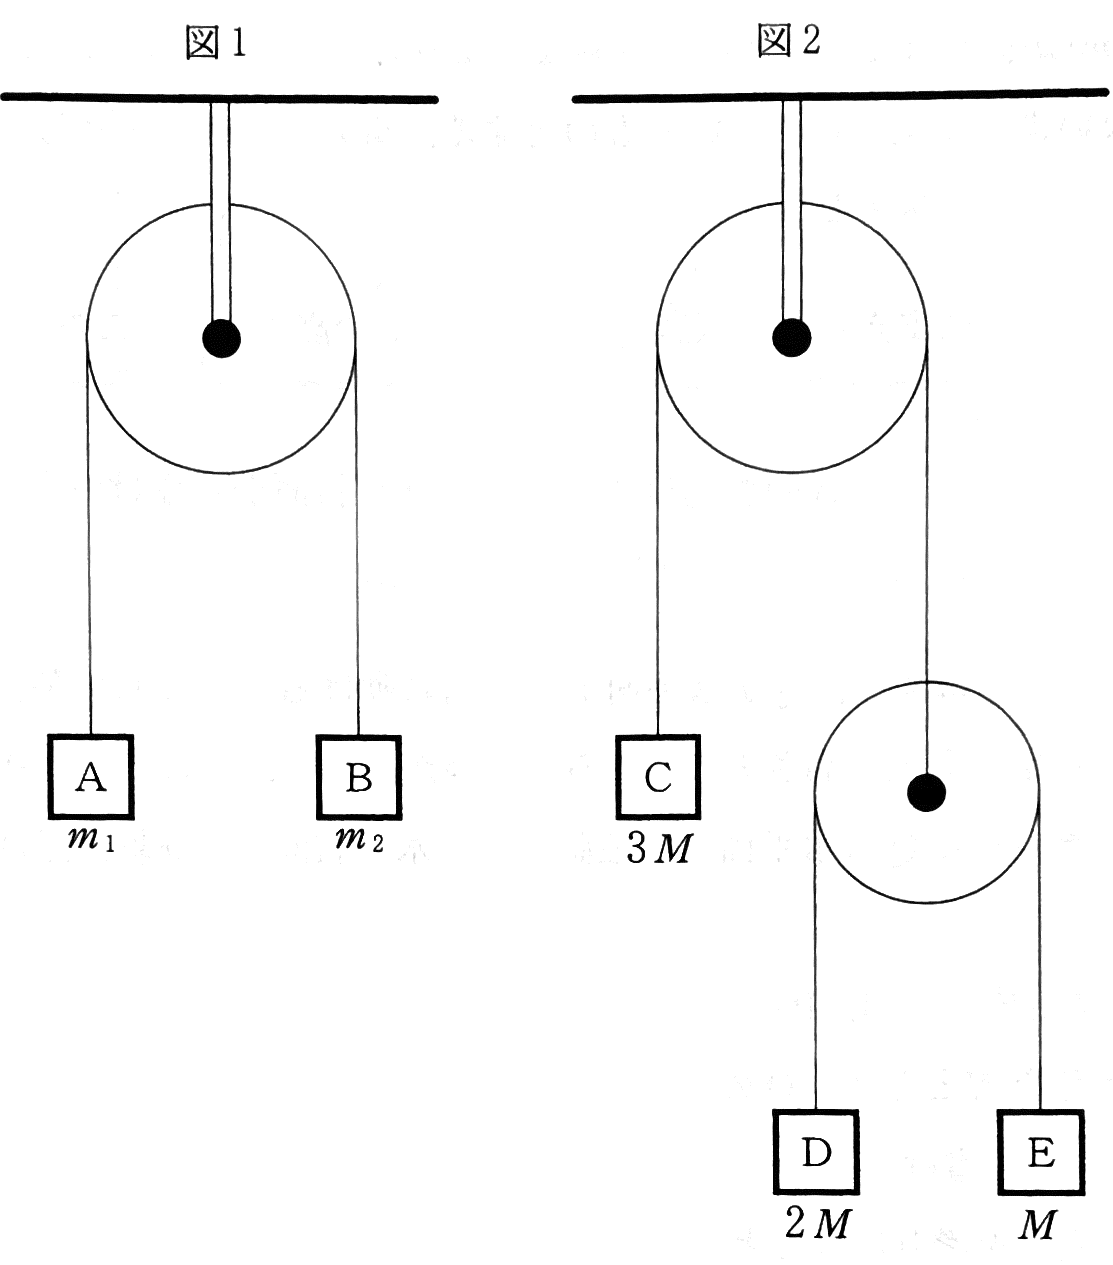
\includegraphics[width=20zw]{../graphs/se_1H_102.png}
\end{figure}


% メモ
\begin{comment}

\end{comment}


%%%%%%%%%%%%%%%%%%

\calcPage

\qPart
%!TEX root = *.tex
%%%%%%%%%%%%%%%%%%
% カウンタのリセット
% 問題文
{
\begin{wrapfigure}{r}{14zw}
  \vspace*{-\intextsep}
  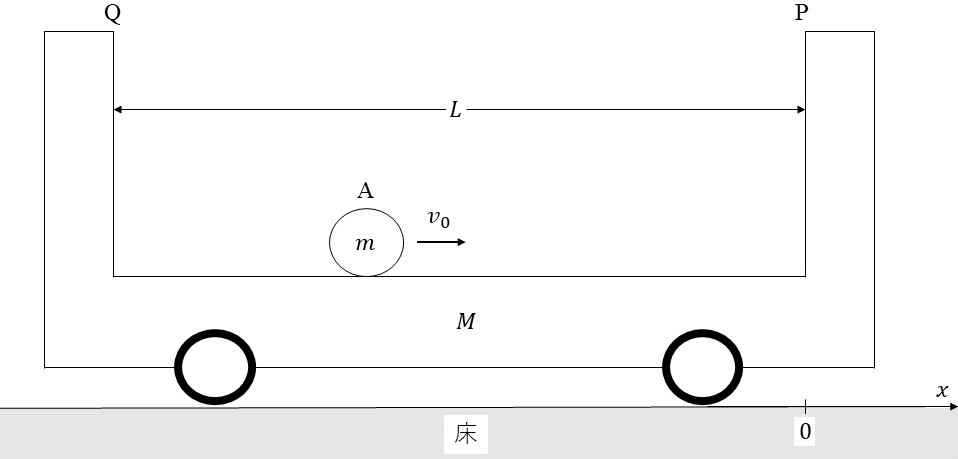
\includegraphics[width=14zw]{../graphs/jumon_42.jpg}
\end{wrapfigure}

図1のように水平な床の上に質量$M$,長さ$L$の台車が静止している.
台車の上には大きさが無視できる質量$m$の小球Aが乗っており,速度$v_0\,(v_0>0)$で運動している.
この問いで使用する速度はすべて床に対する速度であり,麦向きを正とする.
また,摩擦や空気抵抗は無視できるものとする.
\par}

\begin{enumerate}[(1)]
  \setlength{\leftskip}{-1.5zw}
  \setlength{\itemindent}{1zw}\setlength{\labelsep}{0.5zw}
  \setlength{\labelwidth}{1zw}\setlength{\leftmargin}{1zw}
  \setlength{\itemsep}{0.5\baselineskip}
  \item 小球Aが台車両端の壁P,Qに弾性衝突する場合,次の問いに答えよ.
  \begin{enumerate}[(a)]
    \setlength{\leftskip}{-2.5zw}
    \setlength{\itemindent}{1zw}\setlength{\labelsep}{1zw}
    \setlength{\labelwidth}{1zw}
    \item 小球Aが壁Pで最初に台車と衝突した直後の小球および台車の速度(それぞれ$v_1$および$V_1$)を求めよ.
    \item 小球Aは,壁Pで最初に台車と衝突してから時間$T$が経過した後に,壁Qで再び台車と衝突した.このときの時間$T$を求めよ.さらに,壁Qに衝突した直後の小球および台車の速度(それぞれ$v_2$および$V_2$)を求めよ.
    \item $M=m$の場合,小球Aと壁Pの位置の時間変化を$x\mathchar`-t$グラフに実線と点線で示せ.
    ただし,位置は床に固定された座標\x で表し,小球Aが壁Pに最初に衝突した時刻を$t=0$,位置を$x=0$として,$0\leqq t\leqq 3T$の範囲で示せ.
    \item $M=2m$の場合,台車が3Lの距離を進むのに要する時間を求めよ.
  \end{enumerate}
  \item 小球Aが台車両端の壁P,Qに反発係数$e\,(0<e<1)$で非弾性衝突する場合,次の問いに答えよ.
  \begin{enumerate}[(a)]
    \setlength{\leftskip}{-2.5zw}
    \setlength{\itemindent}{1zw}\setlength{\labelsep}{1zw}
    \setlength{\labelwidth}{1zw}
    \item 小球Aが壁Pで最初に台車と衝突した直後の小球および台車の速度(それぞれ${v_1}^\prime$および${V_1}^\prime$)を求めよ.
    \item その後,小球Aは壁Q,Pで台車と衝突をくり返した.2つの壁で合計\nn 回衝突した後の小球および台車の速度(それぞれ${v_n}^\prime$および${V_n}^\prime$)を求めよ.
    \item 十分に時間が経過し,多数の衝突をくり返した後の小球と台車の運動の様子について説明せよ.
  \end{enumerate}
\end{enumerate}



% メモ
\begin{comment}

\end{comment}


%%%%%%%%%%%%%%%%%%

\calcPage

\brankPage

\brankPage

扱った問題やその解答例は\url{https://sh-zoeee.github.io/physics/}で共有します。
下のQRコードからでも辿れます。復習などに役立ててください。
\begin{figure}[htbp]
  \centering
  
\includegraphics[width=0.3\textwidth]{../graphs/qrcode.png}
\end{figure}

共有している各PDFファイルにはパスワードをかけています。開く際には、
nishiuchisatoshi(すべて半角英字)
と入力してください。

\end{document}